\begin{exercises} 

\item \label{Ez:9.4.1}    Let $\vu = 2\vi + \vj$ and $\vv = \vi + 2\vj$ be vectors in $\R^3$.
    \ba
	    \item Without doing any computations, find a unit vector that is orthogonal to both $\vu$ and $\vv$.  What does this tell you about the formula for $\vu \times \vv$?
	    \item Using the bilinearity of the cross product and what you know about cross products involving the fundamental vectors $\vi$ and $\vj$, compute $\vu \times \vv$.
	    \item Next, use the determinant version of Equation~\eqref{E:9.4.cross.def} to compute $\vu \times \vv$.  Write one sentence that compares your results in (a), (b), and (c).
	    \item Find the area of the parallelogram determined by $\vu$ and $\vv$.
    \ea

\begin{exerciseSolution}
    \ba
	    \item Since $\vu$ and $\vv$ lie in the $x$-$y$ plane, the vector $\vk$ is orthogonal to both. So $\vu \times \vv$ is a multiple of $\vk$. 
	    \item The properties of the cross product tell us that 
\begin{align*}
\vu \times \vv &= (2\vi + \vj) \times (\vi + 2\vj) \\
	&= 2(\vi \times \vi) + (\vj \times \vi) + 4(\vi \times \vj) + 2(\vj \times \vj) \\
	&= 2(\vi \times \vi) - (\vi \times \vj) + 4(\vi \times \vj) + 2(\vj \times \vj) \\
	&= 2(\vi \times \vi)  + 3(\vi \times \vj) + 2(\vj \times \vj) \\
	&= 2\vzero + 3\vk + 2\vzero \\
	&= 3 \vk.
\end{align*}
	    \item Using the determinant version of $\vu \times \vv$ we find that 
\[\left| \begin{array}{ccc} \vi & \vj & \vk \\ 2 & 1 & 0 \\ 1 & 2 & 0 \end{array} \right| = [(2)(0)-(0)(1)]\vi - [(1)(0)-(0)(2)] \vj + [(2)(2)-(1)(1)] \vk = 3 \vk.\]
The vectors $\vu$ and $\vv$ lie in the $x$-$y$ plane and a unit vector that is orthogonal to both $\vu$ and $\vv$ is $3 \vk$, established though the determinant formula for the cross product and through the properties of the cross product. 
	    \item The area of the parallelogram determined by $\vu$ and $\vv$ is 
	    \[|\vu \times \vv| = |3\vk| = 3.\]
    \ea
\end{exerciseSolution}

\item \label{Ez:9.4.2}  Let $\vx = \langle 1, 1, 1 \rangle$ and $\vy = \langle 0, 3, -2 \rangle$. 

    \ba
    	\item Are $\vx$ and $\vy$ orthogonal?  Are $\vx$ and $\vy$ parallel?  Clearly explain how you know, using appropriate vector products.
	\item Find a unit vector that is orthogonal to both $\vx$ and $\vy$.
	\item Express $\vy$ as the sum of two vectors:  one parallel to $\vx$, the other orthogonal to $\vx$.
	\item Determine the area of the parallelogram formed by $\vx$ and $\vy$.
    \ea

\begin{exerciseSolution}
  \ba
    \item Two vectors are orthogonal if their dot product is 0. Since $\vx \cdot \vy = 1$, the vectors $\vx$ and $\vy$ are not orthogonal. Vectors $\vx$ and $\vy$ are parallel if one is a scalar multiple of the other, or if their cross product is $\vzero$. Since $\vx \times \vy = -5\vi + 2\vj + 3\vk$, the vectors $\vx$ and $\vy$ are not parallel. 
	\item The vector $\vx \times \vy = -5\vi + 2\vj + 3\vk$ is orthogonal to both $\vx$ and $\vy$, so a unit vector that is orthogonal to both $\vx$ and $\vy$ is $\frac{1}{|\vx \times \vy|} \vx \times \vy = \frac{1}{\sqrt{38}}\langle -5, 2, 3\rangle$. 
	\item The projection 
\[\proj_{\vx} \vy = \frac{\vy \cdot \vx}{\vx \cdot \vx} \vx = \frac{1}{\sqrt{3}}\langle 1,1,1 \rangle\]
of $\vy$ onto $\vx$ is a vector that is parallel to $\vx$, while the vector 
\[\vy - \proj_{\vx} \vy = \frac{1}{\sqrt{3}}\langle -1, 3\sqrt{3}-1, -2\sqrt{3}-1 \rangle\]
is orthogonal to $\vx$. Note that $\vy = \proj_{\vx} \vy + (\vy - \proj_{\vx} \vy)$. 
	\item The area of the parallelogram determined by $\vu$ and $\vv$ is 
	    \[|\vu \times \vv| = | -5\vi + 2\vj + 3\vk| = \sqrt{38}.\]
    \ea
\end{exerciseSolution}

\item \label{Ez:9.4.3}  Consider the triangle in $\R^3$ formed by $P(3, 2, -1)$, $Q(1, -2, 4)$, and $R(4, 4, 0)$.  
%Let $\va = \langle 2, -1, 1 \rangle$ and $\vb = \langle 1, 1, 3 \rangle$.

	\ba
		\item Find $\overrightarrow{PQ}$ and $\overrightarrow{PR}$.
		\item Observe that the area of $\triangle PQR$ is half of the area of the parallelogram formed by $\overrightarrow{PQ}$ and $\overrightarrow{PR}$.  Hence find the area of $\triangle PQR$.
		\item Find a unit vector that is orthogonal to the plane that contains points $P$, $Q$, and $R$.
		\item Determine the measure of $\angle PQR$.
	\ea



\begin{exerciseSolution}
\ba
		\item With the given points $P$, $Q$, and $R$ we have 
\[\overrightarrow{PQ} = \langle -2, -4, 5\rangle  \text{ and } \overrightarrow{PR} = \langle 1, 2, 1 \rangle.\]
		\item The area of the parallelogram formed by $\overrightarrow{PQ}$ and $\overrightarrow{PR}$ is
\[|\overrightarrow{PQ} \times \overrightarrow{PR}| = |\langle -14, 7, 0 \rangle | = \sqrt{245}.\]
Hence the area of $\triangle PQR$ is $\frac{\sqrt{245}}{2}$.
		\item The cross product $\overrightarrow{PQ} \times \overrightarrow{PR}$ is orthogonal to the plane containing $P$, $Q$, and $R$, so a  unit vector that is orthogonal to the plane that contains points $P$, $Q$, and $R$ is 
\[\frac{1}{|\overrightarrow{PQ} \times \overrightarrow{PR}|} \overrightarrow{PQ} \times \overrightarrow{PR} = \frac{1}{\sqrt{245}} \langle -14, 7, 0 \rangle.\]
		\item If $\theta$ is the measure of $\angle PQR$, then 
		\begin{align*}
\theta &= \cos^{-1}\left(\frac{\overrightarrow{QP} \cdot \overrightarrow{QR}}{|\overrightarrow{QP}| |\overrightarrow{QR}|} \right) \\
	&= \cos^{-1}\left(\frac{\langle 2, 4, -5 \rangle \cdot \langle 3, 6, -4 \rangle}{|\langle 2, 4, -5 \rangle| |\langle 3, 6, -4 \rangle|} \right)\\
	&= \cos^{-1}\left(\frac{50}{\sqrt{45} \sqrt{61}} \right) \\
	&\approx 17.38^{\circ}.
\end{align*} 
	\ea
\end{exerciseSolution}



%\item \label{Ez:9.3.1}   

%A tetrahedron is a four-sided solid in $\R^3$, each of whose faces are triangles.  Consider the tetrahedron whose vertices are the points $(1,0,0)$, $(0,1,0)$, $(1,0,0)$, and $(1,1,1)$ as shown in Figure
%\begin{figure}[ht]
%\begin{center}
 %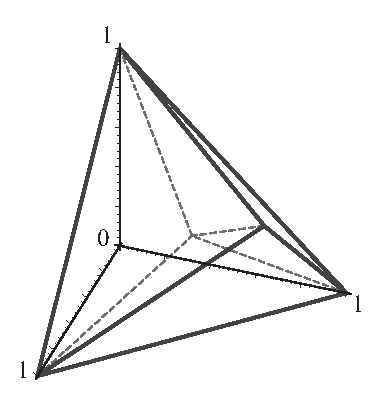
\includegraphics{figures/9_3_Ez1_tetrahedron.eps}
% \caption{The tetrahedron with vertices $(1,0,0)$, $(0,1,0)$, $(1,0,0)$, and $(1,1,1)$.} \label{F:9_3_Ez1_tetrahedron}
%\end{center}
%\end{figure}
%The \emph{centroid} of the tetrahedron is the average of the four vertices, which is the point $(\frac{1}{2}, \frac{1}{2}, \frac{1}{2})$, as shown at the intersection of the dotted lines.
 %   \ba
  %  	\item Consider the face determined by $(1,0,0)$, $(1,1,1)$, and $(0,0,1)$.  Explain why this face is an equilateral triangle.
%	\item 
 %   \ea

%\begin{exerciseSolution}
%\end{exerciseSolution}

\end{exercises}
\afterexercises
